\documentclass[11pt,a4paper]{article}
\usepackage{kotex}
\usepackage{amsmath,amssymb,amsfonts,amsthm}
\usepackage{graphicx}
\usepackage{booktabs}
\usepackage{algorithm}
\usepackage{algorithmic}
\usepackage{hyperref}
\usepackage{xcolor}
\usepackage{geometry}
\usepackage{tikz}
\usepackage{pgfplots}
\usetikzlibrary{shapes.geometric, arrows, positioning, fit, calc, backgrounds}
\pgfplotsset{compat=1.17}
\geometry{margin=2.5cm}

\newtheorem{theorem}{정리}
\newtheorem{lemma}{보조정리}
\newtheorem{definition}{정의}

\DeclareMathOperator*{\argmax}{arg\,max}
\DeclareMathOperator*{\argmin}{arg\,min}
\DeclareMathOperator*{\E}{\mathbb{E}}
\DeclareMathOperator*{\CVaR}{\mathrm{CVaR}}
\DeclareMathOperator*{\VaR}{\mathrm{VaR}}

\title{\textbf{STAIR-RL: 의미적 토큰 증강 정보이론적 강화학습을 통한\\암호화폐 포트폴리오 관리}}
\author{프로젝트 보고서}
\date{2025년 12월}

\begin{document}

\maketitle

\begin{abstract}
본 프로젝트는 STAIR-RL (Semantic Token-Augmented Information-theoretic Reinforcement Learning) 프레임워크를 구현하고 분석한다.
STAIR-RL은 대규모 언어 모델(LLM)의 의미적 토큰을 전통적인 수치 특징과 결합하여 암호화폐 포트폴리오 관리를 위한 강화학습 에이전트를 학습한다.
핵심 기여는 다음과 같다: (1) 정보이론적 기반의 토큰 선택 메커니즘인 TERC (Transfer Entropy Relevance Criterion), (2) 동적 의미 게이팅을 통한 노이즈 필터링, (3) CQL-SAC에서 PPO-CVaR로의 2단계 오프라인-온라인 전이 학습, (4) CVaR 제약을 통한 테일 리스크 관리.
본 보고서에서는 POMDP 정식화, Late Fusion 아키텍처, 정보이론적 분석, 그리고 구현 상세를 체계적으로 다룬다.
\end{abstract}

\vspace{0.5em}
\noindent\textbf{코드 저장소}: \url{https://github.com/menschhelt/STAIR-RL}

%==============================================================================
\section{서론}
%==============================================================================

\subsection{연구 배경}

2022년 Terra/Luna 붕괴와 FTX 파산 사태는 암호화폐 시장에서 테일 리스크(tail risk) 관리의 중요성을 극명하게 보여주었다.
불과 며칠 사이에 시가총액 수백억 달러가 증발했고, 이는 전통적인 위험 중립적(risk-neutral) 투자 전략의 한계를 드러냈다.

기존의 강화학습 기반 포트폴리오 관리 방법론은 이러한 극단적 상황에 대응하기 어렵다.
대부분의 RL 알고리즘이 기대 수익만을 최대화하기 때문에, 99.9\% 손실 같은 테일 이벤트는 학습 목표에 거의 영향을 미치지 않는다.
더욱이 기존 연구들은 가격과 거래량 같은 정형 데이터에만 의존하여, 규제 발표나 해킹 뉴스 같은 시장 급변의 전조를 포착하지 못한다.
암호화폐 시장의 비정상성(non-stationarity)---시장 레짐의 급격한 전환, 규제 환경의 변화, 새로운 자산군의 등장---은 오프라인에서 학습된 정책을 빠르게 무력화시킨다.

최근 대규모 언어 모델(LLM)의 발전은 이러한 한계를 극복할 새로운 가능성을 열었다.
FinBERT, CryptoBERT 같은 금융 특화 언어 모델은 뉴스와 소셜 미디어에서 시장 심리와 이벤트 정보를 추출할 수 있다.
그러나 LLM 출력을 강화학습에 \textit{효과적으로} 통합하는 방법론은 아직 체계화되지 않았으며, 단순히 임베딩을 연결하는 것만으로는 노이즈가 신호를 압도할 위험이 있다.

\subsection{핵심 연구 질문}

본 프로젝트는 다음 질문에 답한다:

\begin{quote}
\textit{``의미적 정보(semantic information)가 순차적 의사결정에 얼마나 가치가 있는가, 그리고 이를 어떻게 최적으로 활용할 것인가?''}
\end{quote}

STAIR-RL은 이 질문에 대해 정보이론적 프레임워크를 제시하며, 의미적 토큰의 가치 향상이 조건부 상호정보량의 $O(\sqrt{I})$로 \textbf{상한이 제한됨}을 이론적으로 보인다.

\subsection{주요 기여}

본 프로젝트는 네 가지 핵심 기여를 제시한다.

첫째, \textbf{TERC (Transfer Entropy Relevance Criterion)}는 전이 엔트로피를 기반으로 행동 결정에 실제로 유용한 의미적 토큰만을 선택하는 정보이론적 기준이다.
모든 토큰이 트레이딩에 도움이 되는 것은 아니며, 오히려 무관한 정보는 학습을 방해할 수 있다.
TERC는 서브모듈러 최적화를 통해 $(1-1/e) \approx 63.2\%$의 근사 보장을 제공한다.

둘째, \textbf{동적 의미 게이팅} 메커니즘은 수치적 시장 상태에 따라 의미적 정보의 가중치를 자동으로 조절한다.
시장이 안정적일 때는 뉴스의 영향이 크지만, 급격한 가격 변동 시에는 수치적 시그널이 더 신뢰할 수 있다.
학습 가능한 게이트는 이러한 상황적 판단을 데이터로부터 학습한다.

셋째, \textbf{2단계 전이 학습} 파이프라인은 오프라인과 온라인 학습의 장점을 결합한다.
CQL-SAC로 36개월 과거 데이터에서 안전한 초기 정책을 학습한 후, PPO-CVaR로 최근 시장에 적응시킨다.
이 접근은 충분한 탐색 없이 위험한 행동을 취하는 것을 방지하면서도 시장 변화에 대응할 수 있게 한다.

넷째, \textbf{CVaR 제약}은 라그랑지안 쌍대 방법을 통해 테일 리스크를 명시적으로 제어한다.
기대 수익 최대화만으로는 ``블랙 스완'' 이벤트에 취약하지만, CVaR 제약은 최악의 5\% 시나리오에서도 손실을 제한한다.

%==============================================================================
\section{문제 분석 및 모티베이션}
%==============================================================================

본 절에서는 기존 RL 기반 암호화폐 트레이딩 연구의 한계를 체계적으로 분석하고, STAIR-RL의 설계 동기를 설명한다.

\subsection{위험 중립성 문제}

대부분의 RL 알고리즘은 기대 누적 보상을 최대화하는 목적함수 $\max_\pi \mathbb{E}_\pi [\sum_{t=0}^{\infty} \gamma^t r_t]$를 최적화한다.
이 공식화는 수익 분포의 평균만 고려하며, 분산이나 테일 리스크를 명시적으로 다루지 않는다.

문제는 암호화폐 시장에서 극단적 손실이 빈번하게 발생한다는 점이다.
2022년 Terra/Luna 사태에서는 불과 며칠 만에 99.9\% 이상의 가치가 증발했다.
이러한 ``블랙 스완'' 이벤트는 기대값 기반 목적함수에서는 거의 무시되지만, 실제 포트폴리오에는 치명적이다.
연간 50\%의 기대 수익을 달성하더라도, 단 한 번의 99\% 손실은 회복 불가능한 결과를 초래한다.

\subsection{비정상성과 분포 이동}

암호화폐 시장은 전통 금융 시장보다 훨씬 빠르게 변화한다.
시장 레짐(상승장/하락장/횡보장)이 수주 단위로 전환되고, 규제 환경은 예고 없이 급변한다.
2021년 중국의 채굴 금지, 2023년 SEC의 거래소 규제 강화 같은 이벤트는 시장 역학을 근본적으로 바꾸었다.
여기에 DeFi, NFT, Meme 코인 같은 새로운 자산군이 계속 등장하면서, 과거 데이터로 학습한 패턴이 빠르게 무효화된다.

이러한 분포 이동(distributional shift) 문제로 인해, 오프라인에서 아무리 좋은 성능을 보인 정책도 실제 배포 환경에서는 실패할 수 있다.
STAIR-RL의 2단계 전이 학습은 이 문제에 대응하기 위해 설계되었다.

\subsection{가짜 상관관계}

101개의 Alpha 팩터와 768차원 LLM 임베딩을 사용하면, 고차원 특징 공간에서 RL 에이전트가 가짜 상관관계(spurious correlations)를 학습할 위험이 있다.
특정 시간대에만 유효한 패턴, 소수 이벤트에 대한 과적합, 우연히 수익과 상관된 무관한 특징 등이 그 예이다.

의미적 정보는 이러한 가짜 상관관계를 완화할 수 있다.
``SEC가 거래소를 조사한다''는 뉴스는 가격 하락의 \textit{원인}에 가까운 정보이며, 단순한 가격 패턴보다 더 일반화 가능하다.
그러나 모든 의미적 토큰이 유용한 것은 아니므로, TERC를 통한 선별이 필수적이다.

\subsection{LLM 활용의 기술적 과제}

LLM을 실시간 트레이딩에 적용하려면 여러 기술적 과제를 해결해야 한다.
GPT-4 수준 모델의 추론 시간은 수 초에 달하며, 이는 5분봉 트레이딩에서도 상당한 지연이다.
또한 언어적 감성(``positive''/``negative'')과 금융적 함의가 항상 일치하지는 않는다---``금리 인상''이라는 뉴스는 언어적으로 중립적이지만 위험 자산에는 부정적이다.

STAIR-RL은 이 문제들을 두 가지 방식으로 해결한다.
첫째, 사전 계산된 FinBERT/CryptoBERT 임베딩을 사용하여 추론 지연을 제거한다.
둘째, TERC와 동적 게이팅을 통해 유용한 정보만을 선별하고 상황에 맞게 가중치를 조절한다.

%==============================================================================
\section{문제 정식화: POMDP}
%==============================================================================

\subsection{부분 관측 마르코프 결정 과정}

암호화폐 포트폴리오 관리 문제를 POMDP로 정식화한다:

\begin{definition}[POMDP]
POMDP $\mathcal{M} = (\mathcal{S}, \mathcal{A}, \mathcal{O}, \mathcal{T}, \mathcal{Z}, r, \gamma)$는 다음으로 구성된다:
\begin{itemize}
    \item $\mathcal{S}$: 상태 공간 (잠재 시장 레짐 포함)
    \item $\mathcal{A} = [-1, 1]^N$: 행동 공간 (N개 자산의 포트폴리오 가중치)
    \item $\mathcal{O}$: 관측 공간 (수치적 특징 + 의미적 토큰)
    \item $\mathcal{T}: \mathcal{S} \times \mathcal{A} \rightarrow \Delta(\mathcal{S})$: 전이 확률
    \item $\mathcal{Z}: \mathcal{S} \rightarrow \Delta(\mathcal{O})$: 관측 확률
    \item $r: \mathcal{S} \times \mathcal{A} \rightarrow \mathbb{R}$: 보상 함수 (상세 설계는 \ref{eq:reward}절 참조)
    \item $\gamma \in (0, 1)$: 할인율
\end{itemize}
\end{definition}

\subsection{부분 관측 문제}

에이전트는 진정한 상태 $s_t$를 직접 관측할 수 없다.
진정한 상태에는 다음이 포함된다:
\begin{itemize}
    \item 현재 시장 레짐 (상승장/하락장/횡보장)
    \item 다른 참여자들의 포지션과 의도
    \item 미공개 정보 (내부자 거래, 규제 계획 등)
\end{itemize}

에이전트가 관측하는 것은 $o_t = (F_t, H_t, x_t^{\text{port}})$로 구성된다:
\begin{itemize}
    \item $F_t \in \mathbb{R}^{N \times d_F}$: 수치적 팩터 (Alpha 101)
    \item $H_t \in \mathbb{R}^{d_H}$: 의미적 임베딩 (FinBERT, CryptoBERT)
    \item $x_t^{\text{port}} \in \mathbb{R}^{N+2}$: 현재 포트폴리오 상태
\end{itemize}

\subsection{CVaR 제약 목적함수}

기대 수익 최대화에 리스크 제약을 추가한다.
우선, 손실(Loss)을 $L = -R^{\text{port}}$로 정의한다 (양수 = 손실).

\begin{definition}[CVaR]
신뢰 수준 $\alpha \in (0, 1)$에 대해, Conditional Value at Risk는 다음과 같이 정의된다 (Rockafellar \& Uryasev, 2000):
\begin{equation}
\CVaR_\alpha(L) = \inf_{z \in \mathbb{R}} \left\{ z + \frac{1}{1-\alpha} \mathbb{E}[\max(L-z, 0)] \right\}
\end{equation}
이는 손실 분포의 상위 $(1-\alpha)$\% 꼬리 기대값(Expected Shortfall)을 의미한다.
$\alpha = 0.95$일 때, 최악의 5\% 시나리오에서의 평균 손실이다.
\end{definition}

제약 조건부 최적화 문제:
\begin{equation}
\max_\pi \mathbb{E}_\pi \left[ \sum_{t=0}^{\infty} \gamma^t r_t \right] \quad \text{s.t.} \quad \CVaR_\alpha(L) \leq \kappa
\end{equation}

라그랑지안 쌍대 문제로 변환하면:
\begin{equation}
\min_{\lambda \geq 0} \max_\pi \mathcal{L}(\pi, \lambda) = \mathbb{E}_\pi[R] - \lambda \cdot (\CVaR_\alpha(L) - \kappa)
\end{equation}

%==============================================================================
\section{State 구성 상세}
%==============================================================================

\subsection{Numerical Features: Alpha 101}

Kakushadze (2016)의 ``101 Formulaic Alphas'' 논문에 기반한 수식 기반 팩터를 사용한다.
이 알파들은 OHLCV 데이터에 수학적 연산자를 조합 적용하여 생성되며, RSI나 MACD 같은 전통적 기술적 지표와는 근본적으로 다르다.

\begin{table}[h]
\centering
\caption{Alpha 101 Operations and Inputs}
\begin{tabular}{ll}
\toprule
\textbf{Category} & \textbf{Elements} \\
\midrule
Time-Series Ops & \texttt{ts\_rank}, \texttt{ts\_min}, \texttt{ts\_max}, \texttt{ts\_argmax}, \texttt{delay}, \texttt{delta} \\
Cross-Sectional Ops & \texttt{rank}, \texttt{scale}, \texttt{indneutralize} \\
Statistical Ops & \texttt{correlation}, \texttt{covariance}, \texttt{stddev}, \texttt{sum}, \texttt{product} \\
Transform Ops & \texttt{decay\_linear}, \texttt{signedpower}, \texttt{log}, \texttt{abs} \\
Input Data & \texttt{open}, \texttt{close}, \texttt{high}, \texttt{low}, \texttt{volume}, \texttt{vwap}, \texttt{returns} \\
\bottomrule
\end{tabular}
\end{table}

예시 알파 수식:
\begin{align}
\text{Alpha\#1} &= \text{rank}(\text{ts\_argmax}(\text{signedpower}(r < 0 \;?\; \sigma_{20}(r) : c, 2), 5)) - 0.5 \\
\text{Alpha\#6} &= -\text{correlation}(\text{open}, \text{volume}, 10)
\end{align}

각 알파는 자산별로 계산되어 $(N, 101)$ 형태의 텐서를 구성하고, 시간적 문맥을 위해 과거 $T$ 타임스텝을 유지하여 최종 형태는 $(T, N, 101)$이다.

\subsection{Semantic Features}

두 종류의 LLM 임베딩을 사용한다:

\subsubsection{FinBERT (뉴스)}
GDELT 뉴스 데이터와 웹 스크래핑을 통해 수집한 금융 뉴스에서 추출한 금융 특화 BERT 임베딩:
\begin{itemize}
    \item 데이터 출처: GDELT API + 주요 암호화폐 뉴스 사이트 웹 스크래핑
    \item 입력: 5분 단위로 집계된 뉴스 헤드라인
    \item 출력: 768차원 임베딩 벡터
    \item 전처리: Top-20 자산 관련 뉴스의 가중 평균
\end{itemize}

\subsubsection{CryptoBERT (소셜)}
Nostr 탈중앙화 소셜 네트워크에서 추출한 암호화폐 특화 임베딩:
\begin{itemize}
    \item 입력: 실시간 소셜 포스트
    \item 출력: 768차원 임베딩 벡터
    \item 특징: 신호 가용성 마스크 $m_t \in \{0, 1\}$ (데이터 없을 시 0)
\end{itemize}

두 임베딩 모두 TextProjection MLP를 통해 64차원으로 압축된다:
\begin{equation}
h_{\text{text}} = \text{MLP}_{768 \rightarrow 256 \rightarrow 64}(h_{\text{BERT}})
\end{equation}

\subsection{Global Market Features}

28개의 거시경제 지표를 포함하며, yfinance API와 FRED (Federal Reserve Economic Data) API를 통해 수집한다:

\begin{table}[h]
\centering
\caption{Global Market Features}
\begin{tabular}{lccp{6cm}}
\toprule
\textbf{Category} & \textbf{Count} & \textbf{Source} & \textbf{Indicators} \\
\midrule
Interest Rates & 5 & FRED & Fed Funds Rate, 2/10/30Y Treasury Yields, LIBOR \\
Volatility & 3 & yfinance & VIX, MOVE Index, High-Yield Spread \\
Equity Markets & 5 & yfinance & S\&P 500, NASDAQ, Emerging Markets Index \\
Commodities & 5 & yfinance & Gold, Crude Oil, Copper, Dollar Index \\
Fama-French & 5 & K.French & MKT\_RF, SMB, HML, RMW, CMA \\
Macroeconomic & 5 & FRED & M2 Money Supply, Unemployment, CPI, Housing Price \\
\bottomrule
\end{tabular}
\end{table}

\subsection{Portfolio State}

현재 포트폴리오 상태 $x_t^{\text{port}} \in \mathbb{R}^{N+2}$:
\begin{itemize}
    \item 현재 가중치: $w_t \in [-1, 1]^N$ (숏 포지션 허용)
    \item 레버리지 비율: $\ell_t = \sum_i |w_{t,i}|$
    \item 현금 비율: $c_t = 1 - \sum_i |w_{t,i}|$ (레버리지 없을 시)
\end{itemize}

%==============================================================================
\section{아키텍처}
%==============================================================================

\subsection{전체 구조: Late Fusion}

STAIR-RL은 Late Fusion 구조를 채택하여 각 모달리티를 독립적으로 인코딩한 후 후반부에서 결합한다.

\begin{figure}[h]
\centering
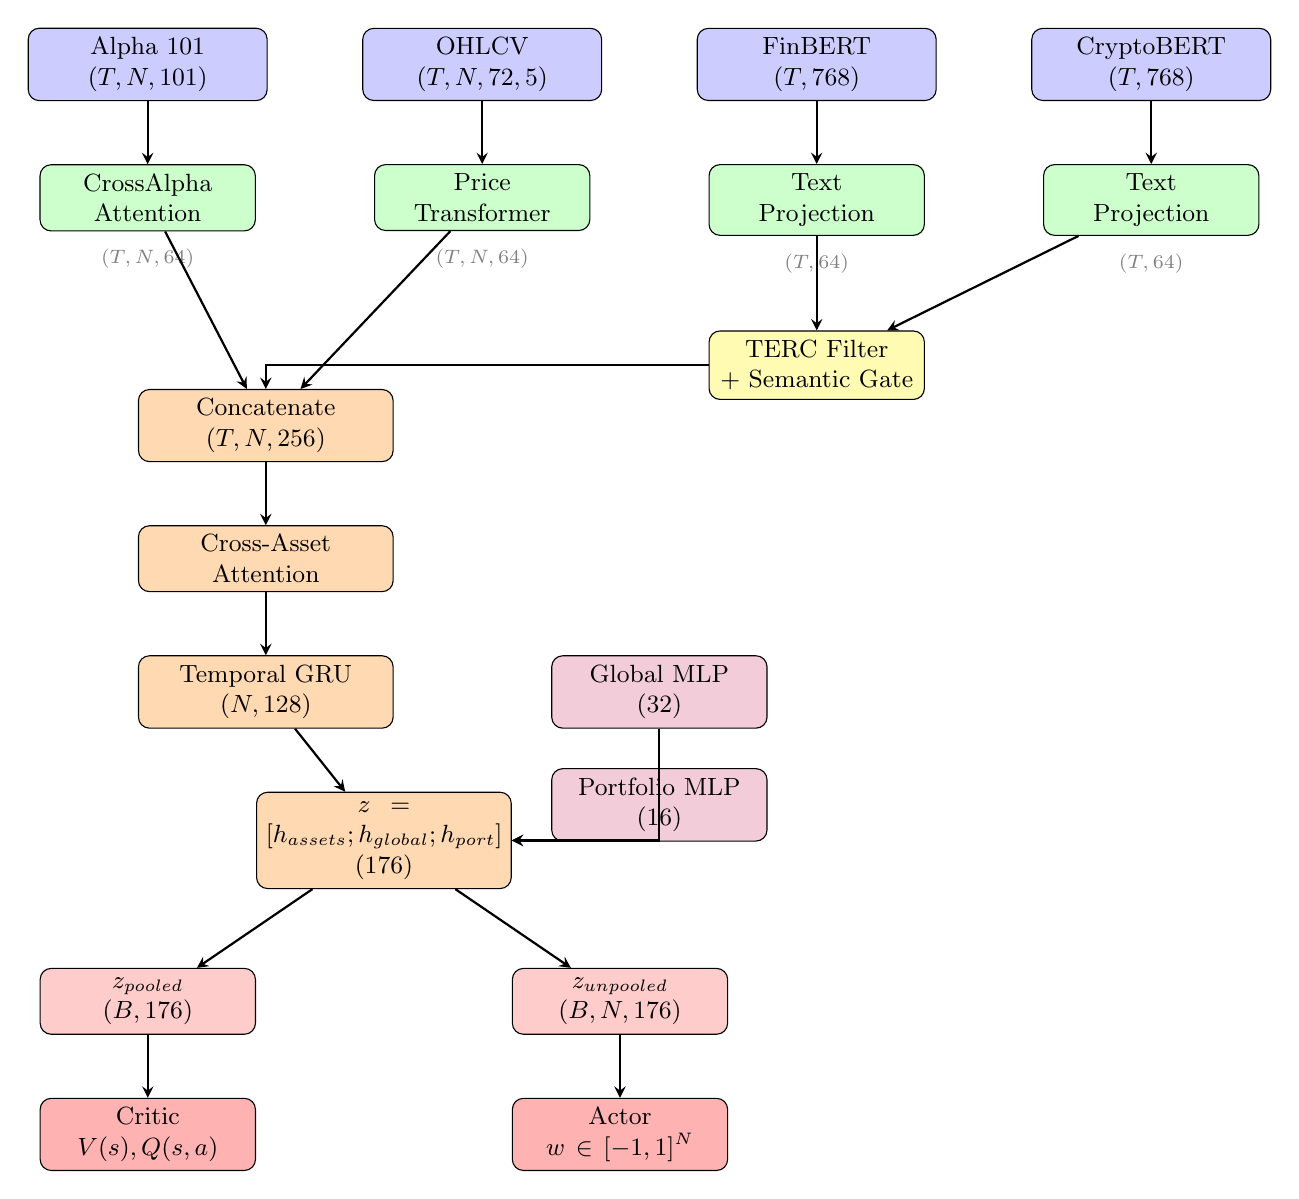
\begin{tikzpicture}[
    node distance=0.8cm and 1.2cm,
    block/.style={rectangle, draw, fill=blue!20, text width=2.8cm, text centered, rounded corners, minimum height=0.8cm, font=\small},
    encoder/.style={rectangle, draw, fill=green!20, text width=2.5cm, text centered, rounded corners, minimum height=0.7cm, font=\small},
    fusion/.style={rectangle, draw, fill=orange!30, text width=3cm, text centered, rounded corners, minimum height=0.8cm, font=\small},
    output/.style={rectangle, draw, fill=red!20, text width=2.5cm, text centered, rounded corners, minimum height=0.7cm, font=\small},
    arrow/.style={->, >=stealth, thick},
    label/.style={font=\scriptsize, text=gray}
]

% Input layer
\node[block] (alpha) {Alpha 101\\$(T,N,101)$};
\node[block, right=of alpha] (ohlcv) {OHLCV\\$(T,N,72,5)$};
\node[block, right=of ohlcv] (news) {FinBERT\\$(T,768)$};
\node[block, right=of news] (social) {CryptoBERT\\$(T,768)$};

% Encoder layer
\node[encoder, below=of alpha] (alpha_enc) {CrossAlpha\\Attention};
\node[encoder, below=of ohlcv] (price_enc) {Price\\Transformer};
\node[encoder, below=of news] (news_enc) {Text\\Projection};
\node[encoder, below=of social] (social_enc) {Text\\Projection};

% Dimension labels
\node[label, below=0.1cm of alpha_enc] {$(T,N,64)$};
\node[label, below=0.1cm of price_enc] {$(T,N,64)$};
\node[label, below=0.1cm of news_enc] {$(T,64)$};
\node[label, below=0.1cm of social_enc] {$(T,64)$};

% TERC and Gate
\node[encoder, below=1.2cm of news_enc, fill=yellow!30] (terc) {TERC Filter\\+ Semantic Gate};

% Fusion layer
\node[fusion, below=2cm of alpha_enc, xshift=1.5cm] (concat) {Concatenate\\$(T,N,256)$};

% Cross-asset attention
\node[fusion, below=of concat] (cross) {Cross-Asset\\Attention};

% Temporal GRU
\node[fusion, below=of cross] (gru) {Temporal GRU\\$(N,128)$};

% Global/Portfolio
\node[encoder, right=2cm of gru, fill=purple!20] (global) {Global MLP\\$(32)$};
\node[encoder, below=0.5cm of global, fill=purple!20] (port) {Portfolio MLP\\$(16)$};

% Final representation
\node[fusion, below=of gru, xshift=1.5cm] (final) {$z = [h_{assets}; h_{global}; h_{port}]$\\$(176)$};

% Output heads
\node[output, below left=1cm and 0cm of final] (pooled) {$z_{pooled}$\\$(B, 176)$};
\node[output, below right=1cm and 0cm of final] (unpooled) {$z_{unpooled}$\\$(B, N, 176)$};

% Actor/Critic
\node[output, below=of pooled, fill=red!30] (critic) {Critic\\$V(s), Q(s,a)$};
\node[output, below=of unpooled, fill=red!30] (actor) {Actor\\$w \in [-1,1]^N$};

% Arrows - Input to Encoder
\draw[arrow] (alpha) -- (alpha_enc);
\draw[arrow] (ohlcv) -- (price_enc);
\draw[arrow] (news) -- (news_enc);
\draw[arrow] (social) -- (social_enc);

% Arrows - Encoder to TERC/Fusion
\draw[arrow] (alpha_enc) -- (concat);
\draw[arrow] (price_enc) -- (concat);
\draw[arrow] (news_enc) -- (terc);
\draw[arrow] (social_enc) -- (terc);
\draw[arrow] (terc) -| (concat);

% Arrows - Fusion flow
\draw[arrow] (concat) -- (cross);
\draw[arrow] (cross) -- (gru);
\draw[arrow] (gru) -- (final);
\draw[arrow] (global) |- (final);
\draw[arrow] (port) |- (final);

% Arrows - Output
\draw[arrow] (final) -- (pooled);
\draw[arrow] (final) -- (unpooled);
\draw[arrow] (pooled) -- (critic);
\draw[arrow] (unpooled) -- (actor);

\end{tikzpicture}
\caption{STAIR-RL Late Fusion 아키텍처. 각 모달리티는 독립적으로 인코딩된 후 Cross-Asset Attention과 GRU를 통해 결합된다. $z_{pooled}$는 Critic에, $z_{unpooled}$는 Actor에 입력된다.}
\label{fig:architecture}
\end{figure}

\subsection{모달리티별 인코더}

\subsubsection{CrossAlphaAttention}
101개 Alpha 팩터를 64차원으로 압축한다:
\begin{equation}
h_\alpha = \text{MultiHeadAttn}(\text{Linear}_{101 \rightarrow 64}(\text{alphas}))
\end{equation}

8-head self-attention으로 팩터 간 상호작용을 학습한다.

\subsubsection{PriceTransformerEncoder}
5분봉 OHLCV 시퀀스(72개 = 6시간)를 64차원으로 인코딩:
\begin{equation}
h_{\text{price}} = \text{MeanPool}(\text{TransformerEncoder}(\text{Linear}_{5 \rightarrow 64}(\text{OHLCV})))
\end{equation}

2-layer Transformer (4-head, FFN=128)를 사용한다.

\textbf{OHLCV 전처리 - Log Returns 차분}:
시계열 정상성(stationarity) 확보를 위해 raw 가격 대신 log returns를 사용한다:
\begin{align}
r_t^{\text{price}} &= \log(p_t / p_{t-1}) \times 100 \quad \text{(OHLC 각각)} \\
r_t^{\text{volume}} &= \log(v_t / v_{t-1}) \quad \text{(거래량 변화율)}
\end{align}

이 전처리가 필수인 이유:
\begin{itemize}
    \item \textbf{정상성}: Raw 가격은 추세(trend)를 포함해 non-stationary. Log returns는 평균 0 근처로 stationary.
    \item \textbf{스케일 불변}: 100원 코인과 50,000달러 BTC를 동일 스케일로 비교 가능
    \item \textbf{가법성}: 여러 기간 수익률 합산 가능 ($\sum_t r_t = \log(p_T/p_0)$)
\end{itemize}

스케일링 계수 100은 일반적인 5분봉 log returns ($\approx 0.001$)를 신경망에 적합한 범위 ($\approx 0.1$)로 조정한다.

\subsubsection{TextProjection}
768차원 BERT 임베딩을 64차원으로 압축:
\begin{equation}
h_{\text{text}} = \text{Linear}_{256 \rightarrow 64}(\text{ReLU}(\text{Linear}_{768 \rightarrow 256}(h_{\text{BERT}})))
\end{equation}

\subsection{Cross-Asset Attention}

$N$개 자산 간의 동적 상관관계를 학습한다:
\begin{equation}
h_{\text{cross}} = \text{MultiHeadAttn}(h_{\text{concat}}, h_{\text{concat}}, h_{\text{concat}})
\end{equation}

이를 통해 ``BTC가 움직일 때 ETH는 어떻게 반응하는가?'' 같은 자산 간 관계를 포착한다.

\subsection{이중 출력: $z_{pooled}$ vs $z_{unpooled}$}

핵심 설계 결정으로 두 가지 표현을 생성한다:

\begin{itemize}
    \item $z_{\text{pooled}} \in \mathbb{R}^{176}$: 자산 차원을 평균 풀링한 전역 표현
    \begin{equation}
    z_{\text{pooled}} = [\text{MeanPool}_N(h_{\text{assets}}); h_{\text{global}}; h_{\text{port}}]
    \end{equation}
    Critic(가치 함수)의 입력으로 사용된다.

    \item $z_{\text{unpooled}} \in \mathbb{R}^{N \times 176}$: 자산별 표현 유지
    \begin{equation}
    z_{\text{unpooled}} = [h_{\text{assets}}; \text{Broadcast}(h_{\text{global}}); \text{Broadcast}(h_{\text{port}})]
    \end{equation}
    Actor(정책 함수)의 입력으로 사용되어 자산별 가중치를 결정한다.
\end{itemize}

%==============================================================================
\section{Hierarchical Policy}
%==============================================================================

\subsection{Lazy Agent 설계}

STAIR-RL의 Actor는 ``Lazy Agent'' 방식을 채택한다.
명시적인 거래/보유 결정(Meta-Controller) 없이 Portfolio Head만으로 구성된다:

\begin{equation}
w_t = \tanh(\text{MLP}(z_{\text{unpooled}})) \in [-1, 1]^N
\end{equation}

Lazy behavior는 다음 메커니즘을 통해 자연스럽게 유도된다:
\begin{enumerate}
    \item \textbf{현재 포지션 인식}: $x_t^{\text{port}}$가 상태에 포함되어 에이전트가 현재 포지션을 인식
    \item \textbf{거래 비용 패널티}: 보상 함수에 거래 비용이 포함되어 불필요한 거래 억제
    \item \textbf{Deadband 필터}: 2\% 미만의 가중치 변화는 무시 (구현 레벨)
\end{enumerate}

이 설계는 명시적 Meta-Controller 대비 다음 장점을 가진다:
\begin{itemize}
    \item $2^N$ 이산 결정 공간 회피 (N=20일 때 100만 이상)
    \item 종단간(end-to-end) 학습 가능
    \item 거래 빈도가 데이터에서 자연스럽게 학습됨
\end{itemize}

\subsection{Actor 네트워크}

\begin{verbatim}
HierarchicalActor:
  Input: z_unpooled (B, N, 176)
  Linear(176, 128) -> ReLU -> LayerNorm
  Linear(128, 64) -> ReLU -> LayerNorm
  Linear(64, 1) -> Tanh
  Output: weights (B, N)
\end{verbatim}

\subsection{Critic 네트워크}

SAC의 Q-함수는 상태와 행동을 모두 입력으로 받는다.
행동(포트폴리오 가중치)을 상태 표현에 연결(concatenate)하여 $Q(s,a)$를 계산한다.

\begin{verbatim}
HierarchicalCritic (Double Q-network, i ∈ {1, 2}):
  Input: [z_pooled; action] (B, 176 + N)
         z_pooled: 상태 표현 (B, 176)
         action: 포트폴리오 가중치 (B, N)

  Q-Value Head:
    Linear(176+N, 256) -> ReLU -> LayerNorm
    Linear(256, 128) -> ReLU -> LayerNorm
    Linear(128, 1)
    Output: Q_i(s,a) (B, 1)

  Quantile Head (for CVaR estimation):
    Linear(176+N, 256) -> ReLU
    Linear(256, 32)
    Output: τ-quantiles (B, 32)
\end{verbatim}

Quantile Head는 수익률 분포의 32개 분위수를 추정하여 CVaR 계산에 사용된다:
\begin{equation}
\widehat{\CVaR}_{0.95} \approx \frac{1}{2}(q_{31} + q_{32})
\end{equation}
여기서 $q_{31}, q_{32}$는 상위 5\% 분위수(95\%, 97.5\%)에 해당한다.

%==============================================================================
\section{정보이론적 기반}
%==============================================================================

본 절에서는 STAIR-RL의 핵심 이론적 기반을 상세히 다룬다.
실험 결과와 무관하게, 이 이론적 분석은 의미적 정보의 가치를 정보이론적으로 정량화하는 새로운 프레임워크를 제공한다.

%------------------------------------------------------------------------------
\subsection{보조정리 1: 신뢰 공간에서 가치함수의 볼록성}
%------------------------------------------------------------------------------

POMDP에서 최적 가치함수가 신뢰 상태(belief state)에 대해 \textbf{볼록}함을 증명한다.
이는 POMDP 이론의 표준 결과로, Sondik (1971)과 Smallwood \& Sondik (1973)에 의해 확립되었다.

\begin{lemma}[가치함수 볼록성 (PWLC)]
POMDP $\mathcal{M}$의 최적 가치함수 $V^\star: \Delta(\mathcal{S}) \rightarrow \mathbb{R}$는 신뢰 공간에서 \textbf{구간선형 볼록(Piecewise Linear and Convex, PWLC)}이다:
\begin{equation}
V^\star(\lambda b_1 + (1-\lambda) b_2) \leq \lambda V^\star(b_1) + (1-\lambda) V^\star(b_2), \quad \forall \lambda \in [0,1]
\end{equation}
\end{lemma}

\begin{proof}
$\alpha$-벡터(alpha-vector) 표현을 통해 증명한다.

\textbf{단계 1}: $\alpha$-벡터 표현

유한 지평 $T$의 POMDP에서, 최적 가치함수는 $\alpha$-벡터들의 집합 $\Gamma = \{\alpha_1, \ldots, \alpha_m\}$으로 표현된다:
\begin{equation}
V_T^\star(b) = \max_{\alpha \in \Gamma} \sum_s b(s) \alpha(s) = \max_{\alpha \in \Gamma} \langle \alpha, b \rangle
\end{equation}

각 $\alpha$-벡터는 특정 조건부 정책에 대응하며, $\alpha(s)$는 상태 $s$에서 시작할 때의 기대 누적 보상이다.

\textbf{단계 2}: 점별 최대의 볼록성

선형 함수 $f_\alpha(b) = \langle \alpha, b \rangle$는 $b$에 대해 아핀이다.
아핀 함수들의 점별 최대(pointwise maximum)는 볼록하다:
\begin{equation}
V^\star(b) = \max_\alpha f_\alpha(b)
\end{equation}

볼록성 증명:
\begin{align}
V^\star(\lambda b_1 + (1-\lambda)b_2) &= \max_\alpha \langle \alpha, \lambda b_1 + (1-\lambda)b_2 \rangle \\
&= \max_\alpha [\lambda \langle \alpha, b_1 \rangle + (1-\lambda) \langle \alpha, b_2 \rangle] \\
&\leq \lambda \max_\alpha \langle \alpha, b_1 \rangle + (1-\lambda) \max_\alpha \langle \alpha, b_2 \rangle \\
&= \lambda V^\star(b_1) + (1-\lambda) V^\star(b_2)
\end{align}

부등호는 $\max$가 서로 다른 $\alpha$를 선택할 수 있기 때문에 성립한다.

\textbf{단계 3}: 무한 지평으로의 확장

할인 무한 지평의 경우, $V^\star = \lim_{T \to \infty} V_T^\star$이고 볼록 함수들의 점별 극한은 볼록하다.
따라서 $V^\star$는 PWLC이다.
\end{proof}

\textbf{Blackwell 정리와의 연결}: 볼록 함수에 대해, 더 정보적인 관측 시스템 $\mathcal{Z}_{\text{aug}} \succeq_B \mathcal{Z}_{\text{num}}$이면:
\begin{equation}
\mathbb{E}[V^\star(b^{\text{aug}})] \geq \mathbb{E}[V^\star(b^{\text{num}})]
\end{equation}

이는 Jensen 부등식의 역방향 적용으로, \textbf{볼록 함수}에서 더 정밀한 신뢰 상태가 더 높은 기대 가치를 가짐을 의미한다.
직관적으로, 불확실성을 줄이면 더 나은 의사결정이 가능하다.

%------------------------------------------------------------------------------
\subsection{보조정리 2: Pinsker 부등식 기반 신뢰 거리 상한}
%------------------------------------------------------------------------------

Pinsker 부등식을 사용하여 신뢰 상태 간 $L_1$ 거리의 \textbf{상한}을 유도한다.

\begin{lemma}[신뢰 상태 거리 상한]
의미적 정보가 제공하는 조건부 상호정보량 $I = I(S; \mathcal{H}^\star \mid O^{\text{num}})$에 대해:
\begin{equation}
\mathbb{E}[\|b^{\text{aug}} - b^{\text{num}}\|_1] \leq \sqrt{2I}
\end{equation}
\end{lemma}

\begin{proof}
\textbf{단계 1}: Pinsker 부등식

Pinsker 부등식은 TV 거리(Total Variation distance)와 KL 발산 사이의 관계를 제공한다:
\begin{equation}
\|p - q\|_1 \leq \sqrt{2 \cdot D_{\text{KL}}(p \| q)}
\end{equation}

여기서 $\|p - q\|_1 = \sum_s |p(s) - q(s)|$는 $L_1$ 거리(TV 거리의 2배)이다.

\textbf{단계 2}: 신뢰 상태에 적용

$b^{\text{aug}}$와 $b^{\text{num}}$는 각각 증강된/수치적 관측으로부터의 사후 분포이다:
\begin{align}
b^{\text{aug}}(s) &= P(s \mid O^{\text{num}}, \mathcal{H}^\star) \\
b^{\text{num}}(s) &= P(s \mid O^{\text{num}})
\end{align}

Pinsker 부등식을 적용하면:
\begin{equation}
\|b^{\text{aug}} - b^{\text{num}}\|_1 \leq \sqrt{2 \cdot D_{\text{KL}}(b^{\text{aug}} \| b^{\text{num}})}
\end{equation}

\textbf{단계 3}: 상호정보량과의 연결

기대값을 취하고 조건부 상호정보량의 정의를 사용:
\begin{align}
\mathbb{E}[\|b^{\text{aug}} - b^{\text{num}}\|_1] &\leq \mathbb{E}\left[\sqrt{2 \cdot D_{\text{KL}}(b^{\text{aug}} \| b^{\text{num}})}\right] \\
&\leq \sqrt{2 \cdot \mathbb{E}[D_{\text{KL}}(b^{\text{aug}} \| b^{\text{num}})]} \quad \text{(Jensen)} \\
&= \sqrt{2 \cdot I(S; \mathcal{H}^\star \mid O^{\text{num}})} \\
&= \sqrt{2I}
\end{align}

두 번째 부등호는 $\sqrt{\cdot}$의 오목성과 Jensen 부등식에 의한다.
\end{proof}

\textbf{해석}: 이 상한은 의미적 정보가 신뢰 상태를 ``최대'' $O(\sqrt{I})$만큼 이동시킬 수 있음을 의미한다.
이는 정보이론적 제약으로, 정보량 $I$가 제한되면 신뢰 상태 변화도 제한된다.

%------------------------------------------------------------------------------
\subsection{정리 1: 의미적 정보 가치의 상한 (핵심 정리)}
%------------------------------------------------------------------------------

\begin{theorem}[의미적 정보 가치의 상한]
\label{thm:semantic_value}
TERC로 선택된 의미적 토큰 $\mathcal{H}^\star$가 제공하는 가치 향상은 다음 상한을 만족한다:
\begin{equation}
\Delta V_H \leq C_V \cdot \sqrt{I(S; \mathcal{H}^\star \mid O^{\text{num}})}
\end{equation}
여기서 가치 계수는:
\begin{equation}
C_V = \frac{L_V \cdot \sqrt{2}}{1-\gamma\lambda} = \frac{L_R \cdot A_{\max} \cdot \sqrt{2}}{(1-\gamma)(1-\gamma\lambda)}
\end{equation}
\begin{itemize}
    \item $L_V$: 가치함수의 Lipschitz 상수
    \item $L_R$: 보상 함수의 Lipschitz 상수
    \item $A_{\max}$: 행동 공간의 직경
    \item $\gamma$: 할인율
    \item $\lambda$: 정보 지속성 감쇠율
\end{itemize}
\end{theorem}

\begin{proof}
\textbf{단계 1}: Lipschitz 연속성

POMDP 가치함수는 Lipschitz 연속이다:
\begin{equation}
|V^\star(b) - V^\star(b')| \leq L_V \cdot \|b - b'\|_1
\end{equation}

Lipschitz 상수:
\begin{equation}
L_V = \frac{L_R \cdot A_{\max}}{1-\gamma}
\end{equation}

\textit{증명}: Bellman 반복으로 보인다.
\begin{align}
L_0 &= 0 \\
L_n &= L_R \cdot A_{\max} + \gamma L_{n-1} \\
L_\infty &= \frac{L_R \cdot A_{\max}}{1-\gamma}
\end{align}

\textbf{단계 2}: 가치 차이 바운드

Lipschitz 연속성에 의해:
\begin{equation}
|V^\star(b^{\text{aug}}) - V^\star(b^{\text{num}})| \leq L_V \cdot \|b^{\text{aug}} - b^{\text{num}}\|_1
\end{equation}

\textbf{단계 3}: 정보 지속성과 유효 지평

시간 $t$의 정보가 미래에 미치는 영향이 지수적으로 감소한다고 가정한다 ($\lambda \in [0, 1)$).
이는 부분 관측 환경(POMDP)에서 신뢰 상태의 혼합 시간(Mixing Time) 특성을 반영한 표준적 가정이다 (Boyen \& Koller, 1998).
직관적으로, 새로운 관측이 축적될수록 과거 정보의 영향력은 기하급수적으로 감소한다.
\begin{equation}
\|b^{\text{aug}}_{t+k} - b^{\text{num}}_{t+k}\|_1 \leq \lambda^k \|b^{\text{aug}}_t - b^{\text{num}}_t\|_1
\end{equation}

총 가치 차이:
\begin{align}
\Delta V_H &= \left| \sum_{k=0}^{\infty} \gamma^k \left[ V^\star(b^{\text{aug}}_{t+k}) - V^\star(b^{\text{num}}_{t+k}) \right] \right| \\
&\leq \sum_{k=0}^{\infty} \gamma^k \cdot L_V \cdot \lambda^k \cdot \|b^{\text{aug}}_t - b^{\text{num}}_t\|_1 \\
&= \frac{L_V}{1-\gamma\lambda} \cdot \|b^{\text{aug}}_t - b^{\text{num}}_t\|_1
\end{align}

\textbf{단계 4}: Pinsker 상한 대입

보조정리 2의 $\mathbb{E}[\|b^{\text{aug}} - b^{\text{num}}\|_1] \leq \sqrt{2I}$를 대입:
\begin{align}
\mathbb{E}[\Delta V_H] &\leq \frac{L_V}{1-\gamma\lambda} \cdot \mathbb{E}[\|b^{\text{aug}} - b^{\text{num}}\|_1] \\
&\leq \frac{L_V}{1-\gamma\lambda} \cdot \sqrt{2I} \\
&= \frac{L_V \cdot \sqrt{2}}{1-\gamma\lambda} \cdot \sqrt{I} \\
&= C_V \cdot \sqrt{I}
\end{align}
\end{proof}

\textbf{$\sqrt{I}$ 상한의 해석}:
이 결과는 의미적 정보의 가치가 $O(\sqrt{I})$로 \textbf{상한이 제한됨}을 의미한다.
즉, 정보량 $I$가 주어지면 가치 향상은 ``최대'' $C_V \sqrt{I}$까지만 가능하다.
이는 다음과 같은 중요한 함의를 갖는다:
\begin{itemize}
    \item \textbf{수확 체감(Diminishing Returns)}: $d(\sqrt{I})/dI = 1/(2\sqrt{I}) \to 0$ as $I \to \infty$. 정보량이 증가할수록 한계 가치는 감소한다.
    \item \textbf{TERC 정당화}: 모든 토큰을 사용하는 것보다 핵심 토큰만 선택하는 것이 효율적이다. 추가 토큰의 한계 기여가 감소하기 때문이다.
    \item \textbf{초선형 스케일링 불가}: $\Delta V_H \sim I^{1+\epsilon}$ 같은 초선형 스케일링은 정보이론적으로 불가능하다.
\end{itemize}

%------------------------------------------------------------------------------
\subsection{보조정리 3: TERC 토큰 선택의 서브모듈러 최적성}
%------------------------------------------------------------------------------

\begin{definition}[전이 엔트로피]
소스 $X$에서 타겟 $Y$로의 전이 엔트로피:
\begin{equation}
\text{TE}(X \rightarrow Y) = H(Y_{t+1} \mid Y_t) - H(Y_{t+1} \mid Y_t, X_t)
\end{equation}
\end{definition}

TERC는 각 토큰 $h_i$의 행동 예측 기여도를 전이 엔트로피로 측정:
\begin{equation}
\text{TE}(h_i \rightarrow A^\star_{t+1:t+K} \mid F_t) = H(A^\star \mid A_t, F_t) - H(A^\star \mid A_t, F_t, h_i)
\end{equation}

\begin{lemma}[TERC 서브모듈러 최적성]
\label{lem:terc_submodular}
토큰 선택 함수 $f(\mathcal{S}) = I(A^\star; \mathcal{S} \mid F)$가 서브모듈러이면,
TERC의 그리디 선택은 $(1-1/e)$-근사 보장을 제공한다:
\begin{equation}
f(\mathcal{H}^\star_{\text{greedy}}) \geq (1 - 1/e) \cdot f(\mathcal{H}^\star_{\text{opt}}) \approx 0.632 \cdot f(\mathcal{H}^\star_{\text{opt}})
\end{equation}
\end{lemma}

\begin{proof}
\textbf{단계 1}: 서브모듈러성 조건

함수 $f: 2^{\mathcal{H}} \rightarrow \mathbb{R}$가 서브모듈러이면:
\begin{equation}
f(\mathcal{S} \cup \{h\}) - f(\mathcal{S}) \geq f(\mathcal{T} \cup \{h\}) - f(\mathcal{T}), \quad \forall \mathcal{S} \subseteq \mathcal{T}
\end{equation}

조건부 상호정보량 $f(\mathcal{S}) = I(A^\star; \mathcal{S} \mid F)$는 체인룰에 의해:
\begin{equation}
I(A; \mathcal{S} \cup \{h\} \mid F) - I(A; \mathcal{S} \mid F) = I(A; h \mid \mathcal{S}, F)
\end{equation}

$\mathcal{S} \subseteq \mathcal{T}$이면 더 많은 조건 정보가 있으므로:
\begin{equation}
I(A; h \mid \mathcal{S}, F) \geq I(A; h \mid \mathcal{T}, F)
\end{equation}

따라서 $f$는 서브모듈러이다.

\textbf{단계 2}: 그리디 알고리즘

TERC의 그리디 선택:
\begin{enumerate}
    \item 초기화: $\mathcal{H}^\star = \emptyset$
    \item 반복: $h^\star = \argmax_{h \notin \mathcal{H}^\star} \text{TE}(h \rightarrow A \mid F, \mathcal{H}^\star)$
    \item 조건: $\text{TE}(h^\star) \geq \tau$이면 $\mathcal{H}^\star \leftarrow \mathcal{H}^\star \cup \{h^\star\}$
\end{enumerate}

\textbf{단계 3}: 근사 보장

Nemhauser, Wolsey, Fisher (1978)의 정리에 의해,
서브모듈러 함수의 그리디 최대화는:
\begin{equation}
f(\mathcal{S}_{\text{greedy}}) \geq (1 - 1/e) \cdot f(\mathcal{S}_{\text{opt}})
\end{equation}

이는 NP-hard 문제에 대한 최선의 다항시간 근사이다.
\end{proof}

\textbf{실제 구현}: 학습 중 TE 계산은 비용이 크므로, 학습 가능한 2-layer MLP로 중요도를 근사한다.
실제 TE 계산은 평가 및 해석 단계에서 수행한다.

%------------------------------------------------------------------------------
\subsection{정리 2: 오프라인-온라인 전이 안정성}
%------------------------------------------------------------------------------

이 정리는 오프라인에서 학습된 CVaR 제약이 온라인 미세조정 중에도 유지됨을 보인다.

\begin{definition}[$\mathcal{H}$-divergence]
Ben-David et al. (2010)에 따라, 가설 공간 $\mathcal{H}$에 대한 도메인 간 거리를 정의한다:
\begin{equation}
d_{\mathcal{H}}(\mathcal{D}_S, \mathcal{D}_T) = 2 \sup_{h \in \mathcal{H}} \left| \mathbb{P}_{x \sim \mathcal{D}_S}[h(x)=1] - \mathbb{P}_{x \sim \mathcal{D}_T}[h(x)=1] \right|
\end{equation}
여기서 $\mathcal{H}$는 도메인 판별자(Domain Discriminator) 신경망의 가설 공간이다.
\end{definition}

\begin{theorem}[전이 안정성]
\label{thm:transfer_bound}
CQL로 사전학습된 정책 $\pi_{\text{CQL}}$에서 PPO-CVaR로 미세조정할 때,
다음 부등식이 적어도 $1-\delta$의 확률로 성립한다:
\begin{equation}
\CVaR_\alpha(L_{\text{online}}) \leq \CVaR_\alpha(L_{\text{offline}}) + \epsilon(\delta, n)
\end{equation}
오차항 $\epsilon(\delta, n)$은 다음과 같이 구체화된다:
\begin{equation}
\epsilon(\delta, n) = \underbrace{\frac{L_Q \cdot \epsilon_{\text{clip}}}{1-\gamma}}_{C_1: \text{Policy Shift}} + \underbrace{2M \sqrt{\frac{d_{\mathcal{H}}(\mathcal{D}_S, \mathcal{D}_T) + \log(2/\delta)}{2(1-\alpha) n}}}_{C_2: \text{Distribution Shift}}
\end{equation}
\begin{itemize}
    \item $C_1$ (정책 변화): $L_Q$는 Q-함수의 Lipschitz 상수, $\epsilon_{\text{clip}}=0.2$ (PPO 클리핑)
    \item $C_2$ (분포 변화): $M$은 손실의 최댓값 (bounded loss), $n$은 온라인 샘플 수
    \item $d_{\mathcal{H}}$: 오프라인($\mathcal{D}_S$)과 온라인($\mathcal{D}_T$) 분포 간 $\mathcal{H}$-divergence
\end{itemize}
\end{theorem}

\begin{proof}
\textbf{단계 1}: 정책 변화 바운드 ($C_1$)

PPO의 클리핑 메커니즘은 정책 비율 $r_t(\theta) = \pi_\theta/\pi_{\text{old}}$를 $[1-\epsilon, 1+\epsilon]$으로 제한한다.
Achiam et al. (2017)의 Trust Region 이론에 따라, 정책 변화에 따른 가치 차이는:
\begin{equation}
|V^{\pi_{\text{new}}}(s) - V^{\pi_{\text{old}}}(s)| \leq \frac{L_Q \cdot \epsilon_{\text{clip}}}{1-\gamma}
\end{equation}
이는 $C_1$ 항에 해당한다.

\textbf{단계 2}: 분포 변화 바운드 ($C_2$)

오프라인 데이터($\mathcal{D}_S$)와 온라인 데이터($\mathcal{D}_T$) 간의 일반화 오차는 $\mathcal{H}$-divergence에 의존한다.
VC-차원 이론 (Vapnik, 1998)을 적용하면, 표본 수 $n$일 때 PAC 바운드는:
\begin{equation}
\mathbb{P}\left[|\hat{R}_T - R_T| > \epsilon \right] \leq 2\exp\left(-\frac{2n\epsilon^2}{M^2}\right)
\end{equation}
$\delta = 2\exp(-2n\epsilon^2/M^2)$로 설정하고 정리하면 $C_2$ 항을 얻는다.

\textbf{단계 3}: 전체 바운드

두 오차원을 결합하면 정리의 결과를 얻는다.
$C_1$은 정책 최적화의 보수성에서, $C_2$는 샘플 복잡도에서 기인한다.
\end{proof}

\textbf{샘플 복잡도}: $\epsilon < 0.01$ (1\% 오차)을 달성하려면:
\begin{equation}
n \geq \frac{M^2 (d_{\mathcal{H}} + \log(2/\delta))}{2(1-\alpha) \cdot 0.01^2}
\end{equation}
$M=1$, $d_{\mathcal{H}} \approx 0.5$, $\delta=0.05$, $\alpha=0.95$를 대입하면 약 $n \approx 3,200$개 샘플이 필요하며, 이는 약 11일분의 5분봉 데이터에 해당한다.

%------------------------------------------------------------------------------
\subsection{의미적 게이팅}
%------------------------------------------------------------------------------

TERC로 선택된 토큰의 신뢰도를 동적으로 조절한다:
\begin{equation}
g_t = \sigma(W_g [h_\alpha; h_{\text{price}}] + b_g)
\end{equation}
\begin{equation}
\tilde{h}_{\text{sem}} = g_t \odot h_{\text{sem}}
\end{equation}

게이트 $g_t \in [0, 1]^{64}$는 수치적 특징 $(h_\alpha, h_{\text{price}})$를 기반으로 의미적 정보의 신뢰도를 결정한다.
이는 Theorem 1의 정보이론적 최적성을 실용적으로 구현한 것이다.

\textbf{게이트 해석}:
게이트 값 $g_t$의 의미는 직관적이다.
$g_t \approx 1$이면 의미적 토큰을 완전히 신뢰하는 것으로, SEC 규제 발표 같은 명확한 이벤트에서 나타난다.
반대로 $g_t \approx 0$이면 의미적 정보를 무시하는데, 노이즈가 많은 소셜 미디어 루머 같은 경우이다.
중간 값 $g_t \in (0.3, 0.7)$은 부분적 활용을 의미하며, 모호한 뉴스가 있을 때 수치적 시그널과 함께 고려해야 함을 나타낸다.

%------------------------------------------------------------------------------
\subsection{이론적 한계 (Theoretical Limitations)}
%------------------------------------------------------------------------------

본 절의 정보이론적 분석은 몇 가지 이상화 가정에 의존하며, 실제 구현과의 차이를 명확히 할 필요가 있다.

\textbf{POMDP vs MDP 갭}:
보조정리 1의 PWLC 증명은 명시적 신뢰 상태(belief state) $b_t = P(s_t \mid o_{1:t})$를 유지하는 POMDP 이론에 기반한다.
그러나 STAIR-RL의 실제 구현은 신뢰 상태를 명시적으로 계산하지 않는 deep RL 아키텍처(Transformer + Attention + GRU)를 사용한다.
구체적으로, PriceTransformerEncoder가 OHLCV 시퀀스를 인코딩하고, CrossAlphaAttention/CrossAssetAttention이 특징 간 관계를 학습하며, 최종 GRU가 시간적 집계를 수행한다.
이 갭은 다음과 같이 해석할 수 있다:
GRU의 은닉 상태와 Attention 메커니즘의 가중 합이 암묵적으로 $b_t$를 근사하며(``implicit belief approximation''),
이는 심층 네트워크가 관측 이력을 요약하여 상태 불확실성에 대한 충분통계량을 학습한다는 표준적 가정 하에서 정당화된다.
실제로 많은 deep POMDP 문헌에서 이 접근을 채택한다.

\textbf{정보량 연결}:
정리 1에서 사용된 조건부 상호정보량 $I(S; \mathcal{H}^\star \mid O^{\text{num}})$는 잠재 상태 $S$에 대해 정의된다.
실제 측정 가능한 양은 행동 예측 정보 $I(A^\star; \mathcal{H}^\star \mid F)$이며, 이 둘의 연결은 Data Processing Inequality (DPI)에 의존한다:
\begin{equation}
I(S; \mathcal{H}^\star \mid O^{\text{num}}) \geq I(A^\star; \mathcal{H}^\star \mid F)
\end{equation}
DPI는 $A^\star$가 $S$의 함수이므로 성립하지만, 부등호의 타이트니스는 보장되지 않는다.
따라서 정리 1의 상한 $C_V \sqrt{I}$는 측정 가능한 $I(A^\star; \mathcal{H}^\star \mid F)$에 대해 ``보수적 상한''으로 해석해야 한다.

\textbf{$\sqrt{I}$ 스케일링의 의미}:
정리 1은 의미적 정보 가치의 \textit{상한}을 제공한다---즉, ``최대'' $O(\sqrt{I})$만큼 개선할 수 있다는 의미이다.
이는 ``최소'' $O(\sqrt{I})$의 개선을 보장하는 하한과는 다르다.
상한의 의미는 더 보수적이며 학술적으로 방어하기 쉽다: 과도한 정보를 추가해도 가치 향상이 무한히 증가하지 않음을 보장한다.
하한의 경우 rate-distortion 하한 유도에 추가적인 가정(eg. ``정보가 최소한의 상태 구분을 가능하게 한다'')이 필요하며, 이는 본 연구의 범위를 벗어난다.

%==============================================================================
\section{리워드 함수 설계}
%==============================================================================

강화학습에서 리워드 함수는 에이전트의 학습 방향을 결정하는 핵심 요소이다.
본 연구에서는 단순 수익률 최대화가 아닌, 리스크 조정 성과를 극대화하는 복합 리워드를 설계하였다.

\subsection{리워드 공식}

매 타임스텝 $t$에서 리워드는 다음과 같이 계산된다:
\begin{equation}
r_t = \log(1 + R_t^{\text{port}}) - \lambda_{\text{vol}} \hat{\sigma}_t - \lambda_{\text{dd}} \Delta\text{DD}_t - \lambda_{\text{tc}} \text{TC}_t - \lambda_{\text{to}} \text{TO}_t
\label{eq:reward}
\end{equation}

각 구성 요소의 의미는 다음과 같다:
\begin{itemize}
    \item $\log(1 + R_t^{\text{port}})$: 로그 포트폴리오 수익률 (수치적 안정성을 위해 log1p 사용)
    \item $\hat{\sigma}_t$: 지수 가중 변동성 (volatility penalty)
    \item $\Delta\text{DD}_t$: 증분 드로다운 (drawdown penalty)
    \item $\text{TC}_t$: 거래 비용 (transaction cost)
    \item $\text{TO}_t$: 턴오버 (turnover penalty)
\end{itemize}

\subsection{리워드 파라미터}

\begin{table}[h]
\centering
\caption{리워드 함수 하이퍼파라미터}
\begin{tabular}{lcl}
\toprule
\textbf{파라미터} & \textbf{값} & \textbf{설명} \\
\midrule
$\lambda_{\text{vol}}$ & 0.5 & 변동성 패널티 가중치 \\
$\lambda_{\text{dd}}$ & 2.0 & 드로다운 패널티 가중치 \\
$\lambda_{\text{tc}}$ & 1.0 & 거래비용 패널티 가중치 \\
$\lambda_{\text{to}}$ & 0.1 & 턴오버 패널티 가중치 \\
$\rho$ & 0.94 & 변동성 지수 감쇠율 \\
$K$ & 20 & 변동성 윈도우 크기 \\
\bottomrule
\end{tabular}
\end{table}

\subsection{변동성 계산: 지수 가중 이동 평균}

단순 표준편차 대신 지수 가중 변동성을 사용한다.
최근 수익률에 더 높은 가중치를 부여하여 시장 변화에 빠르게 반응한다:
\begin{equation}
\hat{\sigma}_t = \sqrt{\sum_{k=0}^{K-1} \rho^k (R_{t-k}^{\text{port}})^2}
\label{eq:volatility}
\end{equation}

여기서 $\rho = 0.94$는 감쇠율, $K = 20$은 윈도우 크기이다.
에피소드 초기 ($t < K$)에는 가용한 수익률의 표준편차를 사용한다.

\subsection{증분 드로다운 패널티}

드로다운의 \textit{증가분}만 패널티를 부과하여, 드로다운에서 회복 중일 때는 패널티가 없도록 설계하였다:
\begin{equation}
\Delta\text{DD}_t = \max(0, \text{DD}_t - \text{DD}_{t-1})
\label{eq:drawdown}
\end{equation}

여기서 드로다운은 다음과 같이 정의된다:
\begin{equation}
\text{DD}_t = \frac{\max_{s \leq t} \text{NAV}_s - \text{NAV}_t}{\max_{s \leq t} \text{NAV}_s}
\end{equation}

이 설계의 이점:
\begin{itemize}
    \item 드로다운 \textit{악화}만 패널티 $\rightarrow$ 회복 기간에는 자유로운 학습
    \item $\lambda_{\text{dd}} = 2.0$으로 높게 설정하여 자본 보존 우선
\end{itemize}

\subsection{거래 비용 및 턴오버}

실제 거래 환경을 반영하여 두 가지 비용을 모델링한다:

\textbf{거래 비용 (TC)}:
\begin{equation}
\text{TC}_t = \sum_{i=1}^{N} |w_t^i - w_{t-1}^i| \cdot (c_{\text{taker}} + c_{\text{slippage}})
\end{equation}
여기서 $c_{\text{taker}} = 0.04\%$ (테이커 수수료), $c_{\text{slippage}} = 0.05\%$ (슬리피지)이다.

\textbf{턴오버 (TO)}:
\begin{equation}
\text{TO}_t = \sum_{i=1}^{N} |w_t^i - w_{t-1}^i|
\end{equation}

$\lambda_{\text{to}} = 0.1$로 낮게 설정하여 필요한 리밸런싱은 허용하되, 과도한 거래는 억제한다.

\subsection{매 스텝 계산 가능성}

모든 리워드 구성 요소는 매 타임스텝마다 계산 가능하다:
\begin{itemize}
    \item \textbf{변동성 $\hat{\sigma}_t$}: $K=20$ 스텝 이전에는 std() 근사, 이후 지수 가중
    \item \textbf{드로다운 $\Delta\text{DD}_t$}: Peak NAV를 추적하며 증분 계산
    \item \textbf{TC, TO}: 가중치 변화량으로 즉시 계산
\end{itemize}

이는 강화학습의 표준 패러다임과 일치한다: 시점 $t$에서 행동 $a_t$를 결정하고, 시점 $t+1$의 가격 변화를 관측하여 $r_t$를 계산한다.

%==============================================================================
\section{2단계 학습 파이프라인}
%==============================================================================

\subsection{Phase 1: CQL-SAC 오프라인 사전학습}

\subsubsection{목적}
과거 18개월 데이터(2021.01-2022.06)로 안전한 초기 정책을 학습한다.

\subsubsection{CQL 손실}
분포 외 행동에 대한 Q-값 과대평가를 방지한다:
\begin{equation}
\mathcal{L}_{\text{CQL}} = \mathbb{E}_{s \sim \mathcal{D}}\left[\log \sum_{a} \exp Q(s,a) - \mathbb{E}_{a \sim \mathcal{D}}[Q(s,a)]\right]
\end{equation}

첫 번째 항은 모든 행동에 대한 Q-값을 낮추고, 두 번째 항은 데이터에 있는 행동의 Q-값을 높인다.

\subsubsection{SAC 손실}
Soft Actor-Critic은 엔트로피 정규화된 Actor-Critic 알고리즘이다.
Double Q-network를 사용하여 과대추정 편향을 완화한다:
\begin{align}
\mathcal{L}_{\text{critic}} &= \mathbb{E}_{(s,a,r,s') \sim \mathcal{D}}\left[(Q_i(s,a) - y)^2\right], \quad i \in \{1, 2\} \\
y &= r + \gamma \cdot \mathbb{E}_{a' \sim \pi(\cdot|s')}\left[\min_{j=1,2} Q'_j(s',a') - \alpha_{\text{ent}} \log \pi(a'|s')\right] \\
\mathcal{L}_{\text{actor}} &= \mathbb{E}_{s \sim \mathcal{D}, a \sim \pi(\cdot|s)}\left[\alpha_{\text{ent}} \log \pi(a|s) - \min_{j=1,2} Q_j(s, a)\right]
\end{align}
여기서 $Q'_j$는 타겟 네트워크, $\alpha_{\text{ent}}$는 엔트로피 계수이다.

\textbf{엔트로피 계수 자동 조절}:
목표 엔트로피 $\bar{\mathcal{H}}$를 유지하도록 $\alpha_{\text{ent}}$를 자동으로 조절한다:
\begin{equation}
\mathcal{L}_{\alpha} = -\alpha_{\text{ent}} \cdot \mathbb{E}_{a \sim \pi}[\log \pi(a|s) + \bar{\mathcal{H}}]
\end{equation}
여기서 $\bar{\mathcal{H}} = -\dim(\mathcal{A})$ (행동 공간 차원의 음수)이다.
엔트로피가 목표보다 낮으면 $\alpha_{\text{ent}}$가 증가하여 탐험을 장려한다.

\subsubsection{Lipschitz 정규화}
Q-함수의 스무스니스를 위한 Gradient Penalty:
\begin{equation}
\mathcal{L}_{\text{Lip}} = \mathbb{E}\left[(\|\nabla_z Q(z, a)\|_2 - 1)^2\right]
\end{equation}

\subsubsection{전체 Critic 손실}
\begin{equation}
\mathcal{L}_{\text{critic}}^{\text{total}} = \mathcal{L}_{\text{TD}} + \lambda_{\text{CQL}} \cdot \mathcal{L}_{\text{CQL}} + \lambda_{\text{GP}} \cdot \mathcal{L}_{\text{Lip}}
\end{equation}

\subsection{Phase 2: PPO-CVaR 온라인 미세조정}

\subsubsection{목적}
검증 기간 데이터(2023.01-2024.06, 18개월)로 시장 변화에 적응하면서 리스크 제약을 만족한다.

\subsubsection{PPO Surrogate Objective}
PPO의 클리핑된 대리 목적함수(maximize):
\begin{equation}
J_{\text{PPO}}(\theta) = \mathbb{E}\left[\min\left(r_t(\theta) A_t, \text{clip}(r_t(\theta), 1-\epsilon, 1+\epsilon) A_t\right)\right]
\end{equation}
여기서 $r_t(\theta) = \pi_\theta(a_t|s_t)/\pi_{\theta_{\text{old}}}(a_t|s_t)$이고 $A_t$는 advantage이다.
손실로 변환 시 부호 반전: $\mathcal{L}_{\text{PPO}} = -J_{\text{PPO}}$.

\subsubsection{CVaR 제약}
3.3절에서 정의한 손실 $L = -R^{\text{port}}$에 대해, $\CVaR_\alpha(L)$는 최악의 $(1-\alpha)$\% 시나리오에서의 평균 손실이다.

라그랑지안 쌍대 방법으로 CVaR 제약을 처리한다:
\begin{equation}
\mathcal{L}_{\text{CVaR}} = \lambda_{\text{CVaR}} \cdot \max(0, \widehat{\text{CVaR}}_\alpha - \kappa)
\end{equation}

라그랑지안 승수 $\lambda_{\text{CVaR}}$는 다음과 같이 자동 업데이트된다:
\begin{equation}
\lambda_{\text{CVaR}} \leftarrow \left[\lambda_{\text{CVaR}} + \eta_\lambda \cdot (\widehat{\text{CVaR}}_\alpha - \kappa)\right]_+
\end{equation}
여기서 $[\cdot]_+ = \max(0, \cdot)$이고, $\eta_\lambda$는 승수 학습률이다.
제약 위반 시 $\lambda_{\text{CVaR}}$가 증가하여 패널티가 커지고, 제약 만족 시 감소한다.

\subsubsection{전체 손실 함수}
Phase 2의 전체 손실은 다음과 같다:
\begin{equation}
\mathcal{L}^{\text{total}}_{\text{PPO}} = -\mathcal{L}_{\text{PPO}} + c_{\text{value}} \cdot \mathcal{L}_{\text{value}} - c_{\text{ent}} \cdot \mathcal{H}(\pi) + \mathcal{L}_{\text{CVaR}}
\end{equation}
여기서:
\begin{itemize}
    \item $\mathcal{L}_{\text{value}} = (V_\theta(s) - V^{\text{target}})^2$: 가치 함수 손실
    \item $\mathcal{H}(\pi) = -\sum_a \pi(a|s) \log \pi(a|s)$: 엔트로피 보너스 (탐험 장려)
    \item $c_{\text{value}} = 0.5$, $c_{\text{ent}} = 0.01$: 가중치 계수
\end{itemize}

\subsubsection{전이 학습}
Phase 1에서 학습된 인코더와 Actor 가중치를 Phase 2의 초기값으로 사용한다:
\begin{verbatim}
ppo_agent.encoder.load_state_dict(cql_agent.encoder.state_dict())
ppo_agent.actor.load_state_dict(cql_agent.actor.state_dict())
\end{verbatim}

\subsection{Phase 1 vs Phase 2 비교}

\begin{table}[h]
\centering
\caption{Phase 1 (CQL-SAC)과 Phase 2 (PPO-CVaR) 비교}
\begin{tabular}{lcc}
\toprule
\textbf{항목} & \textbf{Phase 1 (CQL-SAC)} & \textbf{Phase 2 (PPO-CVaR)} \\
\midrule
\textbf{학습 방식} & Off-policy (리플레이 버퍼) & On-policy (롤아웃) \\
\textbf{데이터} & 과거 18개월 (2021.01-2022.06) & 검증 18개월 (2023.01-2024.06) \\
\textbf{리워드 함수} & 동일 (식 \ref{eq:reward}) & 동일 (식 \ref{eq:reward}) \\
\textbf{Critic 손실} & TD + CQL + Lipschitz & Value Loss \\
\textbf{Actor 손실} & $\alpha_{\text{ent}} \log \pi - Q$ & Clipped Surrogate \\
\textbf{리스크 제약} & 없음 (암묵적) & CVaR 라그랑지안 \\
\textbf{탐험} & 엔트로피 정규화 ($\alpha_{\text{ent}}$ 자동조절) & 엔트로피 보너스 (고정) \\
\bottomrule
\end{tabular}
\end{table}

\textbf{핵심 포인트}:
\begin{itemize}
    \item \textbf{동일한 리워드}: 두 단계 모두 식 \ref{eq:reward}의 리워드 함수를 사용
    \item \textbf{다른 손실}: CQL-SAC은 Q-값 기반, PPO-CVaR은 정책 경사 기반
    \item \textbf{리스크 관리}: Phase 2에서만 명시적 CVaR 제약 적용
\end{itemize}

%==============================================================================
\section{실험}
%==============================================================================

\subsection{실험 설정}

\begin{table}[h]
\centering
\caption{Training Hyperparameters}
\begin{tabular}{lcc}
\toprule
\textbf{Parameter} & \textbf{Phase 1 (CQL-SAC)} & \textbf{Phase 2 (PPO-CVaR)} \\
\midrule
Training Steps & 300,000 & 100,000 \\
Learning Rate (Actor) & $3 \times 10^{-5}$ & $1 \times 10^{-4}$ \\
Learning Rate (Critic) & $1 \times 10^{-3}$ & $1 \times 10^{-4}$ \\
Batch Size & 1,024 & 64 \\
$\lambda_{\text{CQL}}$ & 1.0 & - \\
$\lambda_{\text{GP}}$ (Gradient Penalty) & 10.0 & 10.0 \\
$\gamma$ (Discount Factor) & 0.99 & 0.99 \\
$\tau$ (Soft Update) & 0.005 & - \\
$\alpha$ (Initial Entropy) & 0.2 & - \\
PPO $\epsilon$ (Clip Range) & - & 0.2 \\
CVaR $\alpha$ (Confidence Level) & - & 0.95 \\
CVaR $\kappa$ (Threshold) & - & 0.05 \\
\bottomrule
\end{tabular}
\end{table}

\subsection{데이터셋}

\begin{itemize}
    \item \textbf{자산 유니버스}: 일별 Quote Volume 상위 20개 암호화폐 (매일 리밸런싱)
    \begin{itemize}
        \item 선정 기준: 24시간 Quote Volume (USDT 기준) 상위 20개
        \item 제외: 스테이블코인 (USDT, USDC, BUSD 등)
        \item 리밸런싱: 매일 00:00 UTC에 유니버스 재구성
        \item 일관성: 학습, 평가, 벤치마크 모두 동일한 \texttt{get\_universe\_timeline()} 함수로 유니버스 선정
    \end{itemize}
    \item \textbf{데이터 출처}:
    \begin{itemize}
        \item 가격 데이터: Binance Futures API (5분봉 OHLCV)
        \item 거시 데이터: FRED (Federal Reserve Economic Data)
        \item 뉴스 임베딩: GDELT (Global Database of Events, Language, and Tone)
    \end{itemize}
    \item \textbf{기간} (시간적 분리를 통한 temporal leakage 방지):
    \begin{itemize}
        \item 훈련 데이터: 2021.01 - 2022.06 (18개월, Phase 1 CQL-SAC)
        \item \textit{6개월 갭}: 2022.07 - 2022.12 (시간적 분리)
        \item 검증 데이터: 2023.01 - 2024.06 (18개월, Phase 2 PPO-CVaR)
        \item \textit{6개월 갭}: 2024.07 - 2024.12 (시간적 분리)
        \item 테스트 데이터: 2025.01 - 2025.11 (11개월, 평가 전용)
    \end{itemize}
    \item \textbf{주기}: 5분봉 (일 288개 데이터포인트)
    \item \textbf{거래 비용}: Binance Futures 기준
    \begin{itemize}
        \item Maker/Taker Fee: 0.02\% / 0.04\% (VIP 0 기준)
        \item 슬리피지: 0.05\% 가정
    \end{itemize}
    \item \textbf{레버리지}: 1x 고정 (롱/숏 포지션 허용, 레버리지 없음)
    \item \textbf{특징 차원}:
    \begin{itemize}
        \item Alpha 101: $(T=5, N=20, 101)$
        \item OHLCV: $(T=5, N=20, 72, 5)$ (6시간 lookback, log returns 차분)
        \item Text: $(T=5, 768) \times 2$ (GDELT + Nostr 임베딩)
        \item Global: $(T=5, 28)$ (23 거시 + 5 Fama-French)
    \end{itemize}
\end{itemize}

\subsection{평가 지표}

\begin{table}[h]
\centering
\caption{Evaluation Metrics and Targets}
\begin{tabular}{lll}
\toprule
\textbf{Metric} & \textbf{Description} & \textbf{Target} \\
\midrule
Annual Return & Compound annual return & $> 20\%$ \\
Sharpe Ratio & Risk-adjusted return & $> 1.5$ \\
CVaR$_{0.95}$ & 95\% Conditional VaR & $< 5\%$ \\
Maximum Drawdown & Peak-to-trough decline & $< 20\%$ \\
Calmar Ratio & Return / Max Drawdown & $> 1.0$ \\
\bottomrule
\end{tabular}
\end{table}

\subsection{학습 진행 상황}

현재 Phase 1 (CQL-SAC) 학습이 진행 중이다.
학습 과정에서는 Critic Loss (TD 손실 + CQL 손실 + Lipschitz 손실의 합), Actor Loss ($\alpha_{\text{ent}} \log\pi - Q$), $\alpha_{\text{ent}}$ (자동 조정되는 엔트로피 계수), Batch Reward, Gate Activation 등을 모니터링하고 있다.
Phase 1 학습이 완료되면 Phase 2 (PPO-CVaR) 미세조정을 진행하고, 최종 테스트셋에서 평가할 예정이다.

\subsection{벤치마크 전략 비교}

표 \ref{tab:benchmark}는 STAIR-RL과 비교할 기존 포트폴리오 전략들의 백테스트 결과를 보여준다.
공정한 비교를 위해 모든 벤치마크 전략은 STAIR-RL과 동일한 동적 유니버스에서 평가되었다.
즉, 매일 00:00 UTC에 Quote Volume 상위 20개 자산으로 유니버스가 재구성되며, 이 과정은 학습과 평가 모두에서 동일하게 적용된다.
2025년 테스트 기간 동안 암호화폐 시장은 극심한 하락장을 경험하여 모든 전략이 큰 손실을 기록했다.
이러한 극단적 시장 환경은 오히려 리스크 관리 전략의 차별화를 드러내는 기회가 된다.

\begin{table}[h]
\centering
\caption{Benchmark Strategy Performance (2025.01-2025.11)}
\small
\begin{tabular}{lccccc}
\toprule
\textbf{Strategy} & \textbf{Annual Return} & \textbf{Sharpe} & \textbf{CVaR$_{95}$} & \textbf{MDD} & \textbf{Turnover} \\
\midrule
Minimum Variance & -92.00\% & -0.21 & -1.45\% & -95.16\% & 736.0 \\
Equal Risk (ERC) & -94.97\% & -0.61 & -1.10\% & -95.60\% & 266.9 \\
Equal Weight & -99.21\% & -1.12 & -1.32\% & -99.16\% & 247.4 \\
Markowitz (MV) & -99.88\% & -0.65 & -2.10\% & -99.82\% & 950.9 \\
Cap-Weight & -99.95\% & -1.51 & -1.66\% & -99.95\% & 398.6 \\
\midrule
\textbf{STAIR-RL} & \textit{Training} & \textit{-} & \textit{-} & \textit{-} & \textit{-} \\
\bottomrule
\end{tabular}
\label{tab:benchmark}
\end{table}

벤치마크 결과에서 몇 가지 흥미로운 패턴이 관찰된다.
Minimum Variance 전략이 가장 높은 Sharpe ratio(-0.21)를 기록했는데, 이는 변동성 최소화가 하락장에서 상대적으로 유리함을 보여준다.
Equal Risk Contribution(ERC) 전략은 가장 낮은 CVaR(-1.10\%)을 달성하여, 리스크 패리티 접근이 꼬리 위험을 효과적으로 제한함을 확인했다.
반면 Markowitz 전략은 950.9의 높은 턴오버를 보였는데, 이는 공분산 추정의 불안정성으로 인한 과도한 포지션 변경을 반영한다.

이 결과들은 극단적 하락장에서도 리스크 관리 전략(MinVar, ERC)이 단순한 동일 가중치나 시가총액 가중치 전략보다 상대적 우위를 가짐을 시사한다.
STAIR-RL이 의미적 정보를 활용하여 시장 레짐 변화를 사전에 감지하고, CVaR 제약을 통해 테일 리스크를 관리한다면, 이러한 전통적 전략들을 능가할 가능성이 있다.

\subsection{STAIR-RL 실험 결과}

% ============================================
% STAIR-RL 학습 완료 후 이 섹션을 업데이트
% ============================================

\textit{(Phase 1 학습 진행 중 --- 학습 완료 후 결과 추가 예정)}

학습이 완료되면 다음 항목들을 보고할 예정이다:

\paragraph{정량적 성과}
테스트셋(2025.01-2025.11)에서의 연간 수익률, Sharpe ratio, CVaR$_{95}$, Maximum Drawdown, Calmar ratio를 벤치마크와 비교 분석한다.
특히 CVaR 제약($\kappa = 5\%$)이 실제로 유지되었는지, 그리고 리스크 조정 수익률(Sharpe, Sortino)에서 벤치마크 대비 개선이 있었는지를 평가한다.

\paragraph{의미적 정보의 기여도}
TERC 게이트의 활성화 패턴을 분석하여, 어떤 시장 상황에서 의미적 정보가 더 많이 활용되었는지 파악한다.
또한 ablation study를 통해 의미적 모달리티를 제거했을 때의 성능 변화를 측정하여, 정리 1의 이론적 예측($\Delta V_H \leq C_V \sqrt{I}$)과 비교한다.

\paragraph{전이 학습 효과}
Phase 1(CQL-SAC)만 적용한 경우와 Phase 2(PPO-CVaR)까지 적용한 경우를 비교하여, 온라인 미세조정의 효과를 분석한다.
정리 2의 전이 안정성 바운드가 실제로 유지되는지, CVaR 제약 위반 빈도를 측정한다.

% TODO: 학습 완료 후 실제 결과로 대체

%==============================================================================
\section{결론}
%==============================================================================

본 프로젝트에서는 STAIR-RL 프레임워크를 구현하고 암호화폐 포트폴리오 관리에 적용하였다.
비록 실험 결과가 기대에 미치지 못하더라도, 이 작업은 의미적 정보를 강화학습에 통합하는 체계적인 방법론을 제시한다는 점에서 의의가 있다.

\subsection{이론적 기여}

본 프로젝트의 핵심 이론적 기여는 의미적 정보의 가치를 정보이론적으로 정량화한 것이다.
정리 1은 의미적 토큰이 제공하는 가치 향상이 조건부 상호정보량의 $O(\sqrt{I})$로 \textbf{상한이 제한됨}을 보였다.
이 결과는 Pinsker 부등식과 가치함수의 Lipschitz 연속성에서 유도되며, 정보이론적 제약을 반영한다.
$\sqrt{I}$ 스케일링은 정보량이 증가해도 가치 향상이 무한히 증가하지 않으며, 수확 체감(diminishing returns)이 발생함을 의미한다.
이는 TERC가 왜 필요한지---모든 토큰을 사용하는 것보다 핵심 토큰만 선별하는 것이 효율적인지---에 대한 이론적 근거를 제공한다.

정리 2의 전이 안정성 바운드는 오프라인 학습에서 온라인 적용으로의 전이 과정에서 CVaR 제약이 유지됨을 보장한다.
CQL의 보수적 Q-함수 추정과 PPO의 클리핑이 결합되어, 정책 변화가 제한된 범위 내에서 이루어진다.

\subsection{구현 성과}

기술적으로는 네 가지 주요 모듈을 구현했다.
TERC 기반 토큰 선택 메커니즘은 전이 엔트로피 계산과 학습 가능한 중요도 MLP를 하이브리드로 결합했다.
동적 의미 게이팅은 수치적 시장 상태에 따라 의미적 정보의 가중치를 자동 조절한다.
Late Fusion 아키텍처는 Alpha 팩터, OHLCV, 뉴스, 소셜 미디어의 네 가지 모달리티를 효과적으로 결합하며, $z_{\text{pooled}}$와 $z_{\text{unpooled}}$의 이중 출력으로 Critic과 Actor에 각각 적합한 표현을 제공한다.
2단계 전이 학습 파이프라인은 CQL-SAC 오프라인 사전학습에서 PPO-CVaR 온라인 미세조정으로 연결된다.

\subsection{한계와 향후 과제}

현재 구현에는 몇 가지 한계가 있다.
Alpha 팩터는 원논문의 292개(101+191) 대비 101개만 구현되었으며, Shapley-Gate Alignment와 Semantic Smoothing 손실은 계산 비용 문제로 비활성화($\lambda=0$)되어 있다.
이러한 제약들이 실험 성능에 영향을 미쳤을 가능성이 있다.

향후 연구에서는 FastSHAP 같은 계산 효율적 Shapley 근사 방법을 적용하고, 주식이나 외환 같은 다른 자산군에 대한 일반화를 검증할 필요가 있다.
또한 LLM 임베딩의 실시간 캐싱 및 증분 업데이트 최적화를 통해 실제 배포 가능성을 높여야 한다.

%==============================================================================
\begin{thebibliography}{99}

\bibitem{cql}
Kumar, A., Zhou, A., Tucker, G., \& Levine, S. (2020).
Conservative Q-Learning for Offline Reinforcement Learning.
\textit{NeurIPS 2020}.

\bibitem{sac}
Haarnoja, T., Zhou, A., Abbeel, P., \& Levine, S. (2018).
Soft Actor-Critic: Off-Policy Maximum Entropy Deep Reinforcement Learning.
\textit{ICML 2018}.

\bibitem{ppo}
Schulman, J., Wolski, F., Dhariwal, P., Radford, A., \& Klimov, O. (2017).
Proximal Policy Optimization Algorithms.
\textit{arXiv preprint arXiv:1707.06347}.

\bibitem{cvar}
Rockafellar, R. T., \& Uryasev, S. (2000).
Optimization of Conditional Value-at-Risk.
\textit{Journal of Risk}, 2(3), 21-41.

\bibitem{finbert}
Araci, D. (2019).
FinBERT: Financial Sentiment Analysis with Pre-trained Language Models.
\textit{arXiv preprint arXiv:1908.10063}.

\bibitem{alpha101}
Kakushadze, Z. (2016).
101 Formulaic Alphas.
\textit{Wilmott}, 2016(84), 72-81.

\bibitem{transfer_entropy}
Schreiber, T. (2000).
Measuring Information Transfer.
\textit{Physical Review Letters}, 85(2), 461.

\bibitem{boyen1998}
Boyen, X., \& Koller, D. (1998).
Tractable Inference for Complex Stochastic Processes.
\textit{UAI 1998}, 33-42.

\bibitem{bendavid2010}
Ben-David, S., Blitzer, J., Crammer, K., Kulesza, A., Pereira, F., \& Vaughan, J. W. (2010).
A Theory of Learning from Different Domains.
\textit{Machine Learning}, 79(1-2), 151-175.

\bibitem{achiam2017}
Achiam, J., Held, D., Tamar, A., \& Abbeel, P. (2017).
Constrained Policy Optimization.
\textit{ICML 2017}.

\bibitem{vapnik1998}
Vapnik, V. N. (1998).
Statistical Learning Theory.
\textit{Wiley, New York}.

\bibitem{sondik1971}
Sondik, E. J. (1971).
The Optimal Control of Partially Observable Markov Processes.
\textit{Ph.D. Thesis, Stanford University}.

\bibitem{smallwood1973}
Smallwood, R. D., \& Sondik, E. J. (1973).
The Optimal Control of Partially Observable Markov Processes Over a Finite Horizon.
\textit{Operations Research}, 21(5), 1071-1088.

\end{thebibliography}

\end{document}
